%
% ─── CAPITULO 5: INTRODUCCION A LAS HERRAMIENTAS DE RENDERIZACION ───────────────
%

Durante los capítulos anteriores hemos tratado los fractales desde un punto de vista teórico y matemático, ayudándonos del software \textit{Mathematica} para visualizar imágenes de naturaleza fractal, desde los primeros ejemplos clásicos como el triángulo de Sierpinski o el copo de Koch (imágenes \ref{fig:triangulo-Sierpinski} y \ref{fig:copo-Koch}), representaciones de cuencas de atracción en el capítulo \ref{chap:iteracion}, conjuntos de Julia y Mandelbrot en el capítulo \ref{chap:Julia-Mandelbrot} y atractores de sistemas de funciones iteradas. %TODO referenciar capítulo 4

Queda claro que \textit{Mathematica} es un software de cálculo muy útil, pero también es lento, ya que realmente no está orientado a el renderizado de imágenes. En este sentido, obsérvese que sólo hemos utilizado \textit{Mathematica} para visualizar fractales 2D, que se presentan como subconjuntos del plano euclídeo $\R^2$ o coloreando el plano complejo $\C$. Esto se debe no solo a la simplicidad algoritmica que nos proporciona limitar los razonamientos a 2 dimensiones, sino a que el software es realmente lento en 3 dimensiones.

Sin embargo, y como cabría esperar, existen herramientas que nos ayudan a visualizar las directivas geométricas que nosotros mismos queramos, y además podremos hacerlo a tiempo real. En nuestro caso, utilizaremos la librería \textbf{WebGL}, que es una API de JavaScript para el renderizado de gráficos 2D y 3D dentro de cualquier navegador web. Precisamente este último aspecto es el que nos permitirá desplegar nuestro proyecto en una página web interactiva y accesible desde cualquier dispositivo cuya GPU se lo permita\footnote{Esto se puede comprobar gracias a páginas dedicadas a ello como \href{https://get.webgl.org/}{esta página de testeo WebGL} o \href{http://webglreport.com/}{WebGL Report}}.

WebGL permite que las aplicaciones web utilicen una API basada en \href{https://www.khronos.org/opengles/}{OpenGL ES 2.0} para renderizar imágenes 3D en un elemento \verb|<canvas>| de HTML en los navegadores y sistemas que lo soporten sin necesidad de plug-ins. El principal defecto de herramientas como WebGL es la dificultad a la hora de querer comenzar a visualizar imágenes, pues tiene varios componentes complejos de enlazar en un principio. A continuación explicaremos el flujo de trabajo que utiliza WebGL y cómo podemos comenzar a utilizar la herramienta para visualizar fractales.

\section{Componentes de WebGL}

A grandes rasgos, los programas que utilizan WebGL se componen de código de \verb|JavaScript| que interactúa con la propia biblioteca junto con código \verb|GLSL| que se ejecuta en la GPU. Para dar nuestros primeros pasos con WebGL debemos, en nuestro documento HTML, utilizar un elemento \verb|<canvas>| al cual especificamos sus dimensiones en píxeles. En el siguiente ejemplo, el canvas sería cuadrado de $720\times 720$ píxeles. Evidentemente, a mayor número de píxeles mayor resolución, pero también mayor tiempo de cómputo.

\begin{lstlisting}
<main>
    <canvas id="glCanvas"  width="720" height="720"></canvas>
</main>
\end{lstlisting}

\subsection{Contexto de WebGL}

Por su parte, en JavaScript podemos acceder mediante el DOM al elemento \verb|<canvas>| y extraer un objeto que será lo que a partir de ahora denominemos \textbf{contexto de WebGL} (\verb|WebGLRenderingContext|). Este objeto nos proporciona una interfaz a un contexto de OpenGL ES 2.0 para dibujar en la superficie del canvas, de forma que se pueden invocar muchas de las funciones utilizadas en OpenGL. La forma de extraer este contexto es mediante la función \verb|getContext|:

\begin{lstlisting}
const canvas = document.querySelector("#glCanvas");
// Initialize the GL context
const gl = canvas.getContext("webgl2");

// Only continue if WebGL is available and working
if (gl === null) {
    alert("Unable to initialize WebGL. Your browser or machine may not support it.");
    return;
}
\end{lstlisting}

En caso de éxito, que se tiene en la mayoría de las ocasiones, debemos conservar este objeto, pues será necesario para utilizar la gran mayoría de directivas que implementa WebGL. Los siguientes elementos son los auténticos encargados de los objetos que se renderizan en el canvas.

\subsection{El programa \textit{Shader}}

El `\textbf{shader}' es un programa escrito en el llamado \href{https://www.khronos.org/registry/OpenGL/specs/es/3.2/GLSL_ES_Specification_3.20.pdf}{OpenGL ES Shading Language}, más comúnmente conocido como \textbf{GLSL}, que a partir de la información sobre los vértices que forman una figura genera un color para cada píxel, para así dibujar dicha figura en el canvas. Hay dos tipos de \textit{shader}: el \textbf{vertex shader} y el \textbf{fragment shader}. Ambos se escriben en GLSL, de forma que se le especifica el código GLSL a WebGL y este se ejecuta en la GPU. A continuación se explicarán las principales diferencias entre estos dos componentes.

El \textit{vertex shader} se ejecuta una vez por cada vértice de la figura, su misión es transformar la coordenada de mundo de dicho vértice en coordenadas normalizadas en el intervalo $[-1,1]$, rango utilizado por WebGL en su \href{https://developer.mozilla.org/en-US/docs/Web/API/WebGL_API/WebGL_model_view_projection#clip_space}{clip space}. Tras realizar estos calculos y ajustes, se almacena el valor de salida en la variable \verb|gl_Position|. También podemos utilizar el vertex shader para otros cometidos como calcular la coordenada de textura de un objeto, calcular la normal a un objeto en dicho vértice para posteriormente aplicar algún modelo de iluminación, o cualquier otro procesado que podamos hacer en un vértice con la idea de posteriormente pasarle dicho valor al \textit{fragment shader}.


\begin{figure} [ht]
    \centering
    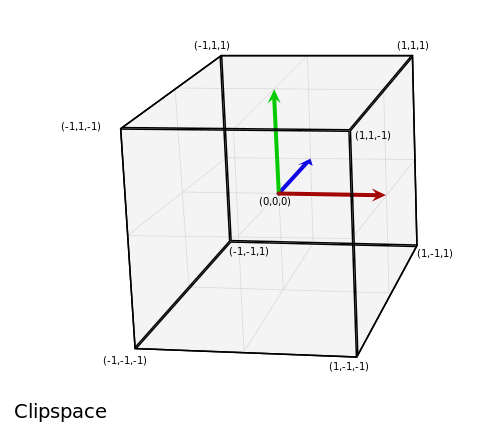
\includegraphics[scale = 0.5]{img/C5/clip-space-graph.png}
    \caption{\textit{Clip space de WebGL}}
    \label{fig:clipspace}
\end{figure}

Por su parte, el \textit{fragment shader}, que es en el que nos centraremos mayormente, es un programa cuyo código se ejecuta una vez por cada píxel y siempre después de que se ejecute el \textit{vertex shader}. Su objetivo es determinar el color del píxel en cuestión en función de la escena que tengamos dibujada, posiblemente aplicando un modelo de iluminación a los objetos que la componen.

El conjunto formado por el \textit{vertex shader} y el \textit{fragment shader} es conocido como \textbf{shader program}, que comúnmente se refiere al mismo únicamente como \textit{shader}. A partir del código fuente de ambos \textit{shaders}, cada uno se crea y compila por separado, para seguidamente unirse en único programa. En el siguiente código se puede ver este procedimiento, siendo el objeto \verb|shaderProgram| el objeto que representa el \textit{programa shader}.

\begin{lstlisting}
// vsSource: Vertex Shader Source Code
// fsSource: Fragment Shader Source Code

const vertexShader   = loadShader(gl, gl.VERTEX_SHADER, 
                                  vsSource);
const fragmentShader = loadShader(gl, gl.FRAGMENT_SHADER, 
                                  fsSource);
  
// Create the shader program

const shaderProgram = gl.createProgram();
gl.attachShader(shaderProgram, vertexShader);
gl.attachShader(shaderProgram, fragmentShader);
gl.linkProgram(shaderProgram);
\end{lstlisting}

Además, GLSL utiliza tres tipos especiales de variables además de las propias variables locales que se definen en el programa, cada una con su cometido, que procedemos a explicar.

\begin{itemize}
    \item \textbf{Variables `attribute'}: Sólo están disponibles en el \textit{vertex shader} y en el código de JavaScript, desde el cual se les da valor. Se suelen utilizar para almacenar información de color, coordenadas de textura, o en general cualquier información que deba ser compartida entre el código de JavaScript y el \textit{vertex shader}.
    \item \textbf{Variables `varying'}: Son declaradas por el \textit{vertex shader} y son utilizadas para enviar información desde el \textit{vertex} para el \textit{fragment shader}, de manera que la información se interpola. Por ejemplo, si el vertex shader asocia color negro a un vértice en una variable \verb|varying| y blanco a otro vértice en la misma variable, entonces los píxeles situados entre estos dos vértices tendrán en esa variable un tono de gris.
    \item \textbf{Variables `uniform'}: Estas variables se definen por el código de JavaScript y se puede acceder a ellas tanto en el \textit{vertex} como en el \textit{fragment shader}. Se usan para especificarle a los shaders valores que no cambian independientemente del vértice o del píxel que se esté ejecutando. Por ejemplo, el color de un material o el zoom que se está aplicando a la escena.
\end{itemize}

Vemos por tanto que mediante estas variables podemos intercambiar información entre el código GLSL que se ejecuta en GPU y el código de JavaScript que comanda el uso de WebGL. Sin embargo, claro está que debe de haber alguna forma de transferir esa información desde JavaScript hasta la GPU. De eso mismo se encargan las estructuras conocidas como \textit{buffers}, que procedemos a explicar.

\subsection{Los \textit{Buffer}}

En el sentido más general de la palabra, un \textit{buffer} es una memoria de almacenamiento temporal de información que permite transferir los datos entre unidades funcionales con características de transferencia diferentes. En nuestro contexto, existen estructuras que almacenan las variables definidas en JavaScript y se transfieren como variables \verb|attribute| o \verb|uniform| al programa \textit{shader}. Por ejemplo, en el siguiente código creamos, a partir de un array de JavaScript que almacena 4 tripletas, cada una representando un color para un vértice, un buffer que las almacena.

\begin{lstlisting}
const colors = [
    1.0,  1.0,  1.0,  1.0,    // white
    1.0,  0.0,  0.0,  1.0,    // red
    0.0,  1.0,  0.0,  1.0,    // green
    0.0,  0.0,  1.0,  1.0,    // blue
];
// Buffer creation
const colorBuffer = gl.createBuffer();
// We select the buffer for the future buffer operations
gl.bindBuffer(gl.ARRAY_BUFFER, colorBuffer);
// We assign the 'colors' array data to the buffer
gl.bufferData(gl.ARRAY_BUFFER, new Float32Array(colors), gl.STATIC_DRAW);
\end{lstlisting}

Y una vez creados los buffers y el \textit{shader} por separado, debemos especificarle al buffer que transfiera la información que contiene a las posiciones de memoria que tiene el \textit{shader} reservadas para las variables que espera. Supongamos que hemos creado en un \textit{vertex shader} una variable \verb|attribute vec4 aVertexColor;| de forma que queremos asociar los colores del código anterior a esta variable por cada uno de los 4 vértices. Mostramos a continuación la forma de hacerlo, pudiendo encontrar más información clarificadora en la documentación de la clase \href{https://developer.mozilla.org/en-US/docs/Web/API/WebGLRenderingContext}{WebGLRenderingContext}.

\begin{lstlisting}
const location = gl.getAttribLocation(shaderProgram, 'aVertexColor');
const numComponents = 4;    // Number of vertex
const type = gl.FLOAT;      // GLSL type of the vars
const normalize = false;    // Do not normalize
const stride = 0;           // Stride
const offset = 0;           // offset

// Select the buffer
gl.bindBuffer(gl.ARRAY_BUFFER, colorBuffer);
gl.vertexAttribPointer(
    location,
    numComponents,
    type,
    normalize,
    stride,
    offset);
gl.enableVertexAttribArray(location);
\end{lstlisting}

De forma muy similar, pero con las funciones correspondientes, se procede desde JavaScript para darle valor a las variables tipo \verb|uniform|.

En nuestro caso particular de visualización de fractales, la característica principal de los mismos es que no se pueden expresar a partir de un conjunto de vértices o líneas, sino que son curvas o superficies totalmente irregulares. Por tanto, a efectos prácticos, nuestro vertex shader tomará como entrada los vértices $(-1,-1)$, $(1,-1)$, $(1,1)$ y $(-1,1)$ y no aplicará ninguna transformación, pues ya están normalizados en el clip space (teniendo en cuenta que estaríamos visualizando un fragmento del plano $z=0$). Cabe en este momento aclarar que en el ámbito de herramientas de renderizado se utiliza el convenio de utilizar la coordenada $Y$ para la altura y la coordenada $Z$ para la profundidad.


